\section{Definitions}

A \emph{MAPF instance} $\inst$ is a pair $(G,A)$, where $G$ is a graph $G = (V,E)$ and $A$ is a set of agents. An agent $a_i \in A$ is a pair $a_i = (s_i,g_i)$, where $s_i \in V$ is the start location and $g_i \in V$ is the goal location of agent $a_i$.

Our task is to find a \emph{valid plan} $\pi_i$ for each agent $a_i \in A$ being a valid path from $s_i$ to $g_i$. We use $\pi_i(t) = v$ to denote that agent $a_i$ is located at vertex $v$ at timestep $t$. Time is discrete and at each timestep, an agent can either wait at its current location or move to a neighboring location.
%
Furthermore, we require that each pair of plans $\pi_i$ and $\pi_j$, $i \neq j$ is collision-free. Based on MAPF terminology~\cite{stern2019mapfVarians}, there are five types of collisions. % (see Figure~\ref{fig:conflict_def}).
Here, we forbid \emph{edge}, \emph{vertex}, and \emph{swap} conflicts while allowing \emph{follow} and \emph{cycle} conflicts since the two latter prevent agents from occupying the same location. Note, however, that all of our methods work in any setting.%We call this setting \emph{parallel motion}, as opposed to \emph{pebble motion}~\cite{pebble_motion}, where all of the conflicts are forbidden.
%
%\begin{figure}[ht]
%\centering
%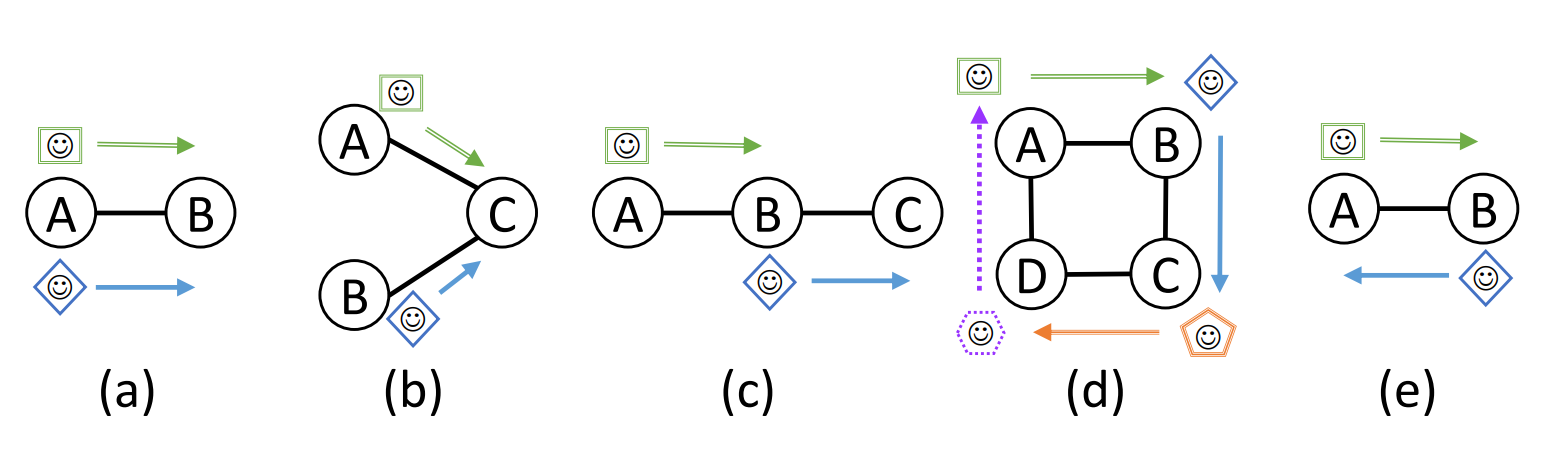
\includegraphics[width=0.99\columnwidth]{img/conflicts.PNG}
%\caption{Conflicts between two or more agents. (a) \emph{edge conflict}, (b) \emph{vertex conflict}, (c) \emph{following conflict}, (d) \emph{cycle conflict}, (e) \emph{swapping conflict}. Figure taken from~\cite{stern2019mapfVarians}.}
%\label{fig:conflict_def}
%\end{figure}

We are interested in \emph{makespan} optimal solutions. Makespan (or horizon) refers to the length of a plan. % Once an agent arrives at its goal location it does not disappear.
% An agent may move out of the goal location again, however,
A plan ends once all of the agents are at the goal location at the same time. This means that the length of the plan $|\pi_i|$ is the same for all of the agents. Another common cost function is \emph{sum of costs}~\cite{ICTS_soc}. Note that finding an optimal solution for either of the cost functions is an NP-hard problem~\cite{NP-hard1,NP-hard2}.

%%% Local Variables:
%%% mode: latex
%%% TeX-master: "main"
%%% End:
